
The product is constructed with a number of components, which all have a central role of the final product. They can all be seen in \autoref{fig:sys_dia}. A list of the major components and their function can be seen below  

\begin{itemize}[noitemsep] 
\item \gls{mcu}: The central part of any integrated system, handles all the calculations and the program code.
\item Radio: All the communications with the rest of the world will be handled by the radio, sending on the VHF and UHF band.
\item \gls{imu}: Movement detection is measured with a accelerometer, this to determine if the unit is  in motion or laying still. 
\item \gls{ldo}: A Low-dropout regulator can supply the system with a smoother voltage because no switching is acctualy taking place.
\item Hall sensor: The hall sensor is used as a switch for the system by sensing if a magnet is nearby and then turning off the circuit.
\item \gls{rtc}: A real time clock is important to aquire data at a specific set time, it is important that the clock is exact over the whole life of the pruduct.
\end{itemize} 


\begin{figure}[H] 
\centering 
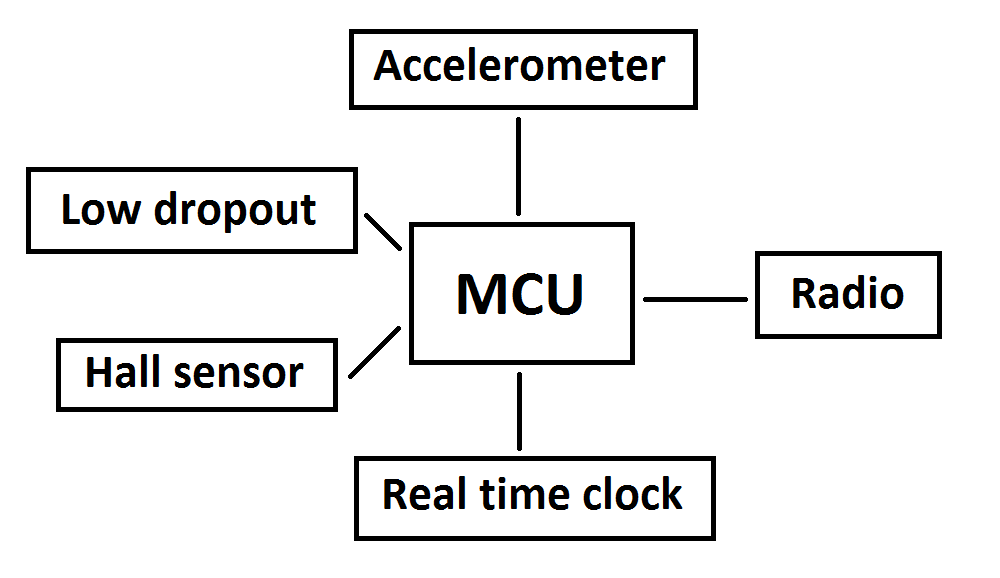
\includegraphics[width=.8\linewidth]{Figures/System_diagram} 
\captionsource{The prototype connection}{Aurthor}
\label{fig:sys_dia} 
\end{figure} 

Each of the components in this project is carfully chosen to get the functionallity and effect that the company is after. To ensure the system works as intended the company have aquired development boards to each of the components. Every components needs to be tested to ensure their induvidial functionallity. Each development board is connected to the micro controllers board. First off the gls{mcu} have to be set up in a correct way with all it parameters and then the other components could be connected and initilized one after another. The whole connection can be seen in \autoref{rattbo}

\begin{figure}[H] 
\centering 
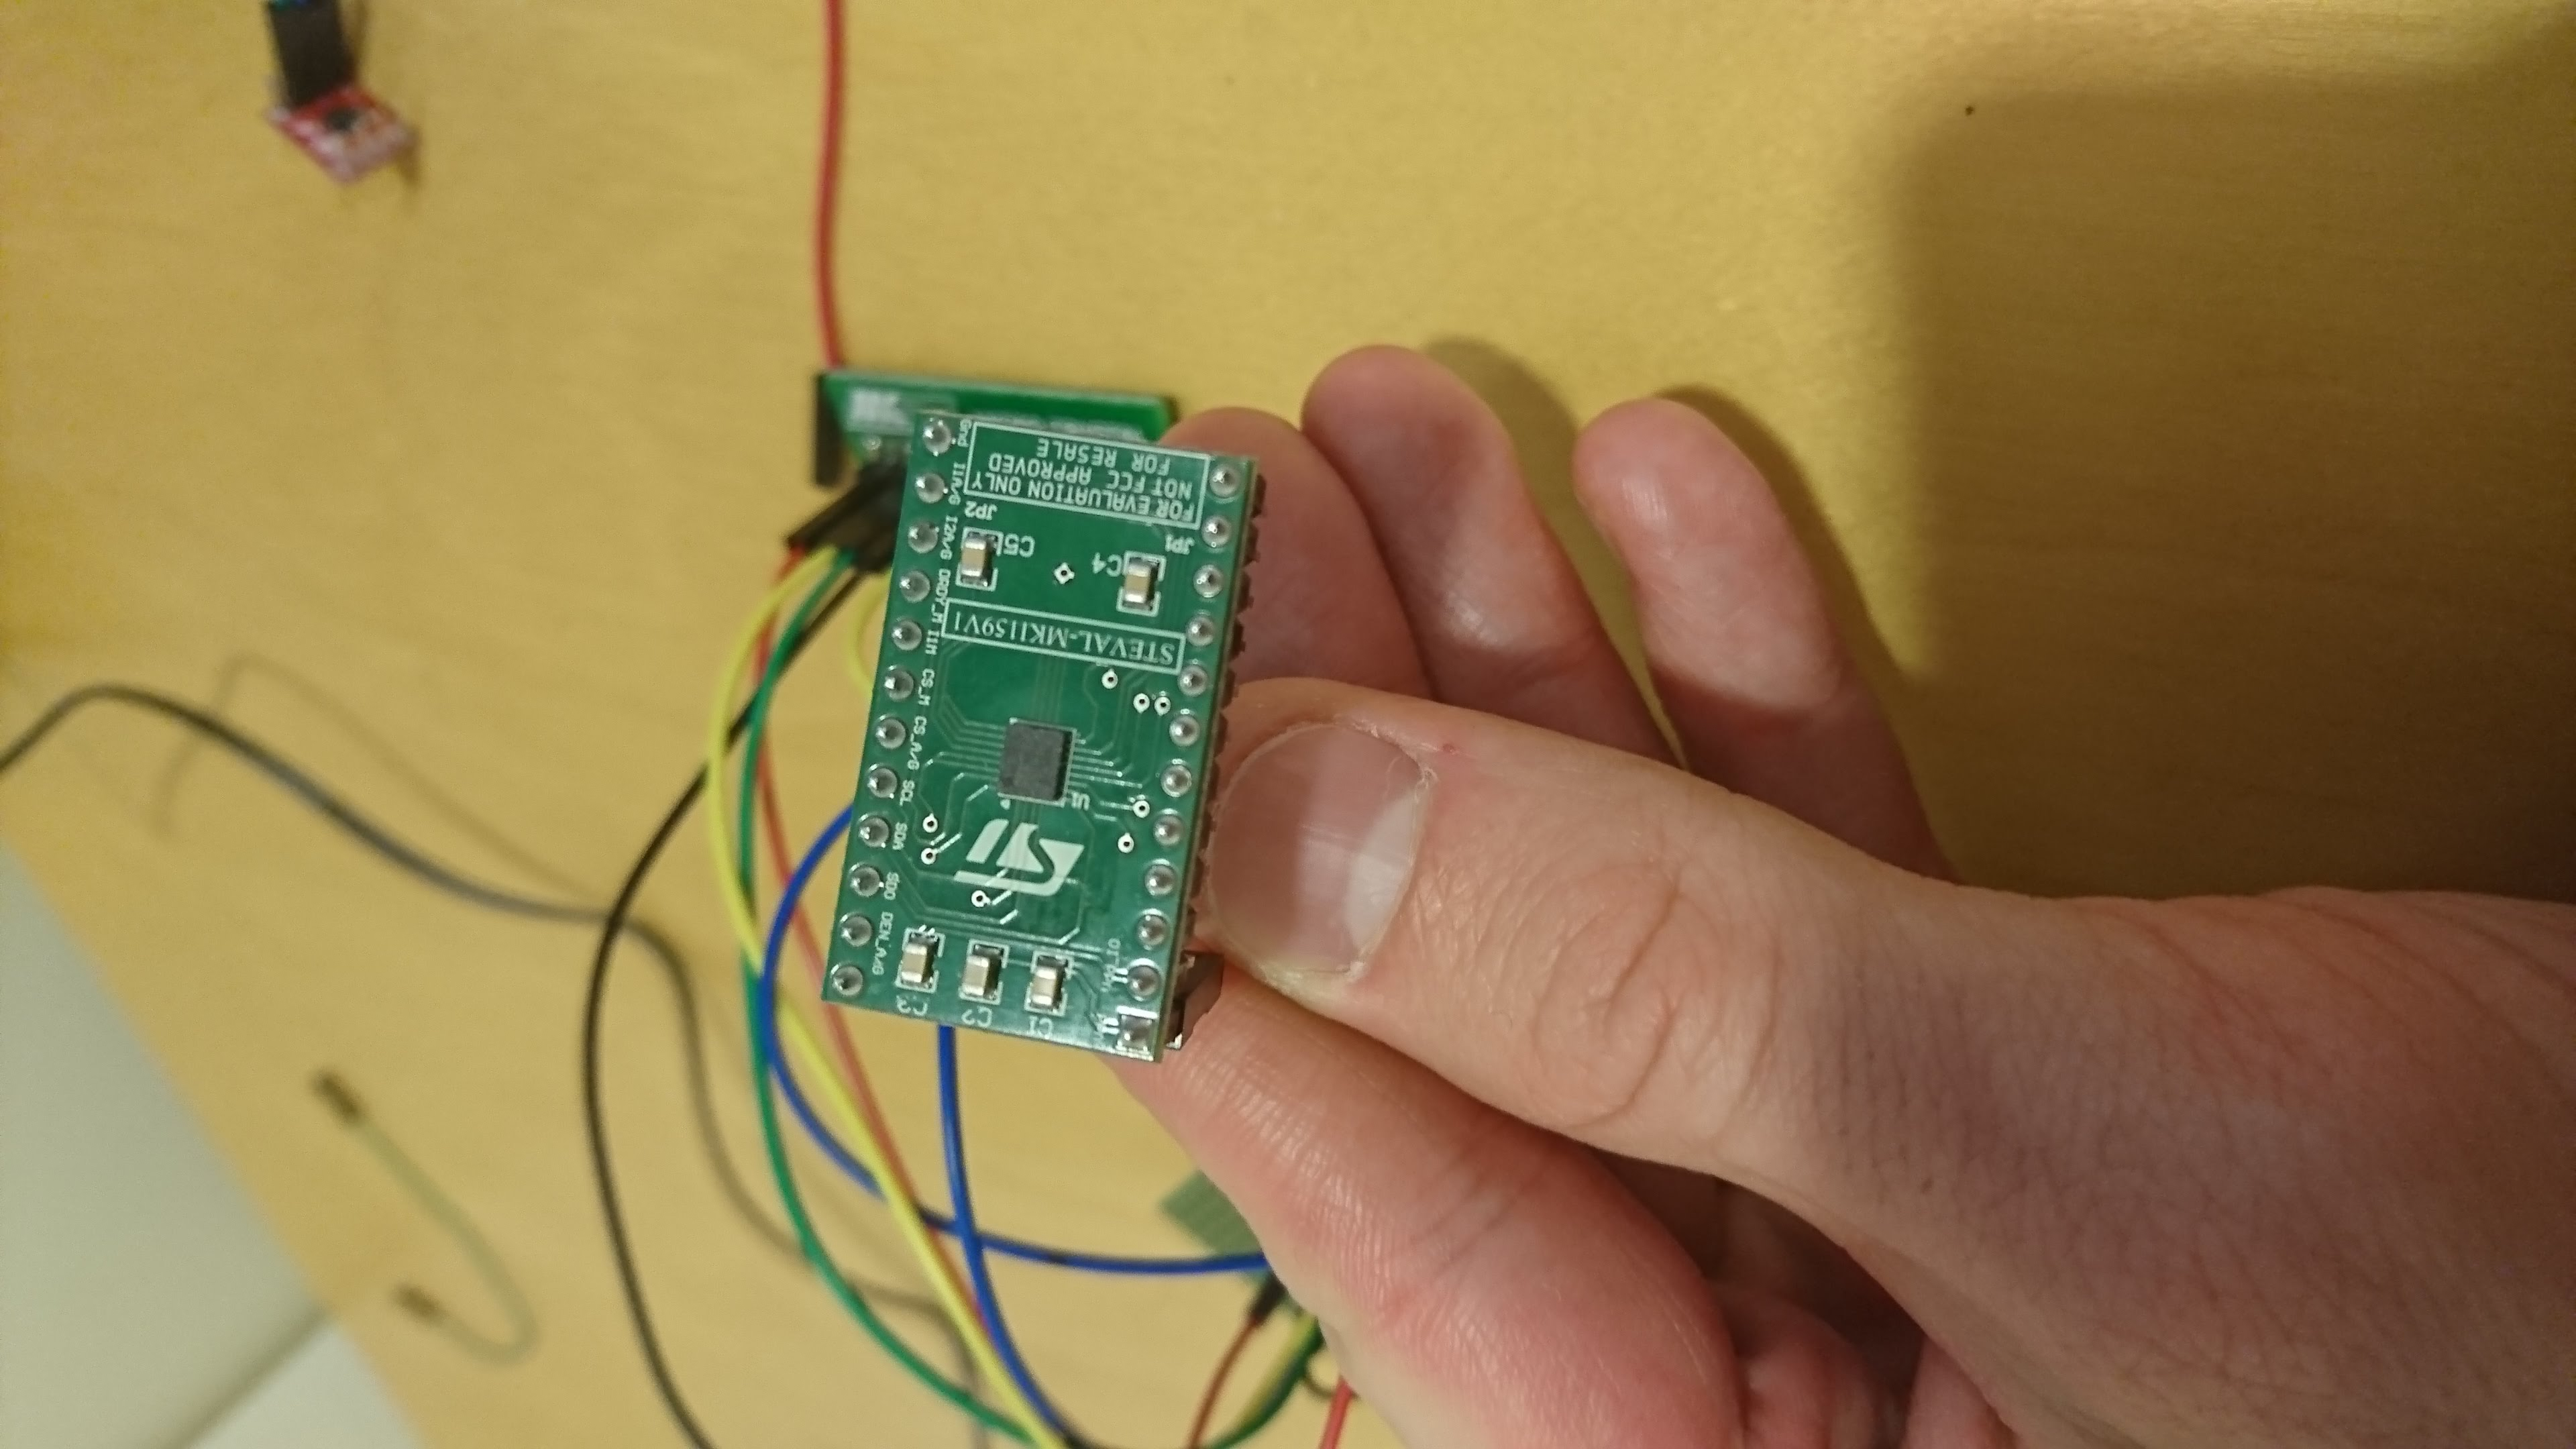
\includegraphics[width=.8\linewidth]{Figures/DSC_0103} 
\captionsource{The prototype connection}{\url{Aurthor}}
\label{rattbo} 
\end{figure} 

The \gls{mcu} can dtad

\subsection{MCU}
The \gls{mcu} used for this project is a processor type that is used by this company many times before and has been chosen to this project for its small size, low power draw, sufficient connections and feautures. It is a pic18lf45k22\cite{pic18}.


\subsection{Accelerometer}
The accelerometer used is a 
